
%% \section{Evaluation}

%% \TODO{Link to repository. Along with instructions \texttt{;)}}

%% How it improves processing time of embeddings over wikidata.

%% How it allows users to get approximate query results on wikidata
%% queries that would otherwise time-out on public endpoints. 

\section{Demonstration Plan}

 \begin{figure*}
   \centering
   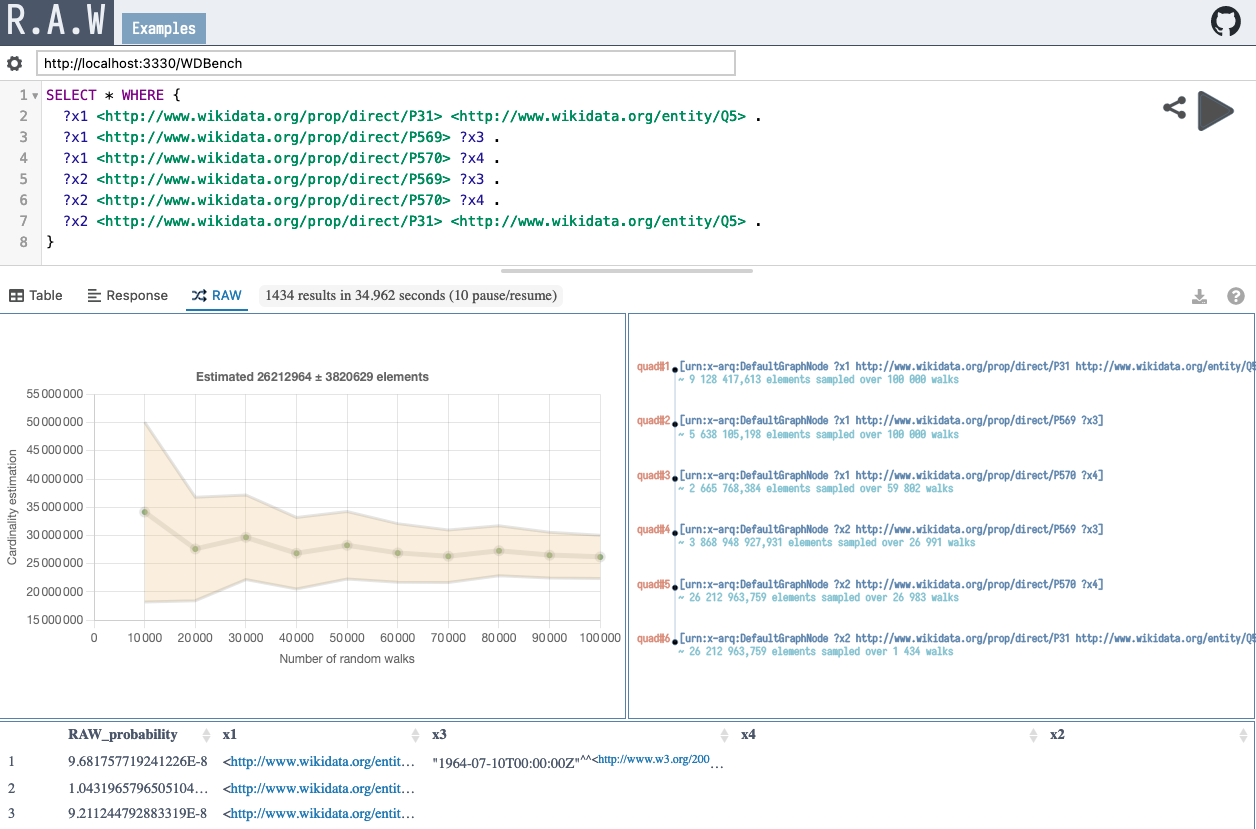
\includegraphics[width=0.85\textwidth]{figures/raw_screenshot.png}
   \caption{\label{fig:raw_screenshot}User interface of \NAME providing useful insights on the query.}
 \end{figure*}

%\paragraph{Target audience.}
%Researchers and practitioners in need of sampling services over RDF
%knowledge graphs. \TODO{In fields.}

 As a motivating example, we rely on the query 604 of
 WDbench~\cite{angles2022wdbench} presented in
 Figure~\ref{fig:raw_screenshot}. This query searches for people
 with the same date of birth and death. This query returns ~25M results,
 time-out on the public Wikidata SPARQL endpoint, and takes more than
 2 hours to complete on JENA. However, using \NAME, in 35 seconds it
 is possible to estimate that the query should return around $26 \pm 3$ 
 millions of results and return 1434 random results.

 
% \paragraph{Web interface.}
Figure~\ref{fig:raw_screenshot} presents the user interface exploiting
\NAME's random walks. The top part of the figure shows where the users
type their queries. By pressing the play button, it asks the server
for random walks on this whole BGP. When the server reaches a
configurable threshold of $10 000$ random walks, or $60s$ of execution
time, it returns its results. By repeating the operation, results are
merged iteratively in a pay-as-you-go fashion hence displaying more
accurate information. Figure~\ref{fig:raw_screenshot} shows that over
$10$ iterations, \NAME performed $100k$ random walks but only $1434$
succeeded, i.e. found a solution mappings. Yet, the bottom left figure provides an estimate
of the number of results over the number of random walks with % over the number of random walks??
confidence intervals. The bottom right figure provides the estimated
number of intermediate results along with the number of random walks
that reached each triple/quad pattern.  Finally, the bottom part shows
both failed and succeeded random walks along with the probability that
they were chosen at execution time.

\paragraph{Getting insights on timed out WDBench queries.}
A few queries of WDBench fail to execute under the 60 seconds mark,
providing nothing whatsoever. We execute these queries using \NAME and
show that, with as little as 1 second, we retrieve interesting
insights on the query plan that may help optimizers to perform their
join ordering. We also get a rough approximation of the number of
results that we improve by executing the query for additional seconds.
The plotted curve converges towards the actual cardinality of the query.
